%%%%%%%%%%%%%%%%%%%%%%%%%%%%%%%%%%%%%%%%%%%%%%%%%%%%%%%%%%%%%%%%%%%%%%
% How to use writeLaTeX: 
%
% You edit the source code here on the left, and the preview on the
% right shows you the result within a few seconds.
%
% Bookmark this page and share the URL with your co-authors. They can
% edit at the same time!
%
% You can upload figures, bibliographies, custom classes and
% styles using the files menu.
%
%%%%%%%%%%%%%%%%%%%%%%%%%%%%%%%%%%%%%%%%%%%%%%%%%%%%%%%%%%%%%%%%%%%%%%

\documentclass[12pt]{article}

\usepackage{sbc-template}
\usepackage{placeins}
\usepackage{graphicx,url}
\renewcommand{\figurename}{}


%\usepackage[brazil]{babel}   
\usepackage[utf8]{inputenc}  

     
\sloppy

\title{Trabalho Prático - Projeto e Análise de Algoritmos}

\author{Thiago Gomes Martins, Henrique Mendonça Castelar Campos}

\address{Ciência da Computação -- Pontifícia Universidade Católica de Minas Gerais (PUC MG)}

\begin{document} 

\maketitle

\begin{abstract}
  Optimization problems are common across various sectors, including the planning of industrial or commercial facility locations. This study addresses the challenge faced by a network of stores in opening multiple franchises, minimizing installation costs, and maintaining a minimum distance between stores to avoid internal competition. We implement brute-force and branch-and-bound approaches to explore configurations and eliminate unproductive solutions, respectively. The comparative analysis evaluates the effectiveness and processing times of both strategies for franchise location planning.
\end{abstract}
     
\begin{resumo} 
  Problemas de otimização são comuns em diversos setores, incluindo o planejamento de localização de instalações industriais ou comerciais. Este estudo aborda o desafio enfrentado por uma rede de lojas na abertura de várias franquias, minimizando custos de instalação e mantendo uma distância mínima entre as lojas para evitar concorrência interna. Implementamos abordagens por força bruta e branch-and-bound para explorar configurações e eliminar soluções improdutivas, respectivamente. A análise comparativa avalia a eficácia e os tempos de processamento de ambas as estratégias para o planejamento de localização de franquias.
\end{resumo}


\section{Introdução}

\paragraph{}Otimização de problemas é uma área fundamental em diversos setores, desempenhando um papel crucial no desenvolvimento e na eficiência de processos industriais, comerciais e logísticos. Um dos desafios mais comuns nesse campo é o planejamento da localização de instalações, como lojas, fábricas ou centros de distribuição, dentro de uma determinada região. A decisão de onde posicionar essas instalações pode ter um impacto significativo nos custos operacionais, na eficiência da cadeia de suprimentos e na satisfação do cliente.

\paragraph{}Este artigo aborda especificamente o problema de localização de franquias de uma rede de lojas, considerando a minimização dos custos de instalação e a necessidade de manter uma distância mínima entre as lojas para evitar competição interna. A otimização dessa localização é essencial para garantir o sucesso e a sustentabilidade do negócio, equilibrando a acessibilidade para os clientes, os custos de operação e a viabilidade financeira das franquias.

\paragraph{}Neste contexto, são apresentadas duas abordagens para resolver o problema de localização das franquias: uma solução por força bruta, que explora todas as configurações possı́veis, e um método de branch-and-bound, que busca aprimorar a eficiência da solução por meio da eliminação de soluções improdutivas. Será realizada uma análise comparativa entre esses métodos, avaliando não apenas a qualidade das soluções encontradas, mas também os tempos de processamento e a escalabilidade para problemas de maior complexidade

\paragraph{}Por meio deste estudo, busca-se fornecer insights valiosos para redes de lojas e empresas interessadas em otimizar a localização de suas instalações, contribuindo para a melhoria dos processos de tomada de decisão e para o aumento da eficiência operacional.

\section{Solução proposta}

\paragraph{}A resolução desse problema consiste em gerar subconjuntos por meio da adição de cada ponto informado pelo usuário. O subconjunto que estiver de acordo com a restrição e com o critério de otimização, será considerado como a melhor solução para esse problema. A restrição é a distância mínima permitida entre as lojas e o fato de somente existir uma loja por franqueado. E o critério de otimização é o número de franquias ser o maior possível, e o custo total de instalação, o menor possível.

\paragraph{}Um dos algoritmos utilizados é o algoritmo da Força Bruta, que consiste em gerar todas as soluções possíveis e escolher a melhor das que atendem à restrição e o critério de otimização. Para isso, serão gerados todos os subconjuntos do conjunto de pontos candidatos, e aquele subconjunto que estiver de acordo com a restrição (distância mínima) e for o melhor, será considerado como a melhor solução.

\paragraph{}Outro algoritmo utilizado é o algoritmo Branch and Bound, que consiste em recursivamente gerar subconjuntos do conjunto dos pontos candidatos, por meio da adição e da não adição do elemento analisado. Caso o elemento analisado não atenda a restrição, ele não será adicionado e nem comparado a melhor solução, e nem serão gerados filhos dele. Caso ele atenda a restrição, e tenha terminado a recursão, ele será comparado com a melhor solução até então. Caso ele seja melhor que a melhor solução, ou não exista até então uma melhor solução, ele será considerado como a melhor solução. O algoritmo pára quando o índice de recursão for igual ao número máximo de franquias.

\paragraph{}Na análise do consumo de memória, ambos algoritmos, no pior caso, gastaram 
\(f(n)=2^n\), que é o espaço gasto para armazenar todas os vetores possíveis. Já no processamento o algoritmo da Força Bruta gastou \(f(n)=2^(^n^+^1^)-2\), e o Branch and Bound \(f(n)=3*2^(^n^-^1^)+1\).

\section{Implementação}

\paragraph{}A implementação da solução de software para resolução de problemas de otimização foi feita na linguagem de programação Java. Para isso, foram criados três pacotes (\textit{packages}): modelo, visão e controlador, seguindo o padrão \textit{Model View Controller}.

\paragraph{}No pacote modelo, estão as classes:

\begin{itemize}
    \item \textit{PontoCandidato}, que armazena os dados de um ponto que se pensa instalar uma loja; 
    \item \textit{ListaPontosCandidatos} que armazena em um dicionário (\textit{Dictionary}) com todos os pontos candidatos;
    \item \textit{Algoritmo} que define os atributos e métodos que uma classe que executa um algoritmo de otimização deve implementar;
    \item \textit{BranchAndBound} que implementa o algoritmo de otimização Branch-and-Bound;
    \item \textit{ForcaBruta} que implementa o algoritmo de otimização Força-Bruta;
    \item \textit{Solucao} que implementa atributos e métodos utilizados na verificação da qualidade de uma solução.
\end{itemize}

\paragraph{}No pacote visão, estão as classes:

\begin{itemize}
    \item \textit{FuncoesGraficas} que contém métodos estáticos para obtenção da resolução da tela;
    \item \textit{GerarCor} que contém método estático para gerar cor com base em um índice;
    \item \textit{IncreaseDecreaseJTextField}, que implementa um \textit{JTextField} com botões de incrementar e decrementar o valor numérico;
    \item \textit{JanelaArquivo}, utilizado na abertura e salvamento de arquivos;
    \item \textit{JanelaDistanciaMinima}, que implementa uma janela para obter do usuário a distância mínima permitida entre dois pontos (lojas) escolhidos;
    \item \textit{JanelaGerarDados}, que implementa uma janela para obter do usuário a quantidade de franquias e a quantidade de lojas por franquia que ele deseja gerar;
    \item \textit{JanelaPrincipal}, que implementa a janela principal do programa;
    \item \textit{JanelaResultados}, que mostra os resultados da execução dos algoritmos. 
\end{itemize}

\paragraph{}E no pacote controlador, estão as classes:

\begin{itemize}
    \item \textit{ControladorJanela}, responsável por controlar o funcionamento do programa quando estiver no modo com interface gráfica;
    \item \textit{ControladorLinhaComando}, responsável por controlar o funcionamento do programa no modo linha de comando.
\end{itemize}

\paragraph{}O desenvolvimento de interfaces gráficas foi feito por meio do uso das bibliotecas \textit{Java Swing} e \textit{Java Awt}, nativas da linguagem Java. Para este programa foram desenvolvidas seis janelas:

\begin{itemize}
    \item a janela principal, que é a primeira janela a ser exibida para o usuário, e quando gerado a solução nela é desenhado o mapa;
    \item janela para geração de dados aleatórios, que mostra a opção para o usuário selecionar o número de franquias e o número de lojas por franquia;
    \item janela de resultados, que mostra uma tabela com os pontos (lojas) selecionados (número de franquia, coordenadas, custo e cor do ícone no mapa);
    \item janela para abertura de arquivos, que permite o usuário selecionar o arquivo que ele deseja abrir;
    \item janela para salvamento de arquivos, que permite o usuário selecionar a pasta e o nome que deseja utilizar para salvar um arquivo;
    \item janela para configuração da mínima distância permitida, que permite o usuário definir a mínima distância permitida entre os pontos escolhidos.
\end{itemize}

\begin{figure}[H]
    \centering
    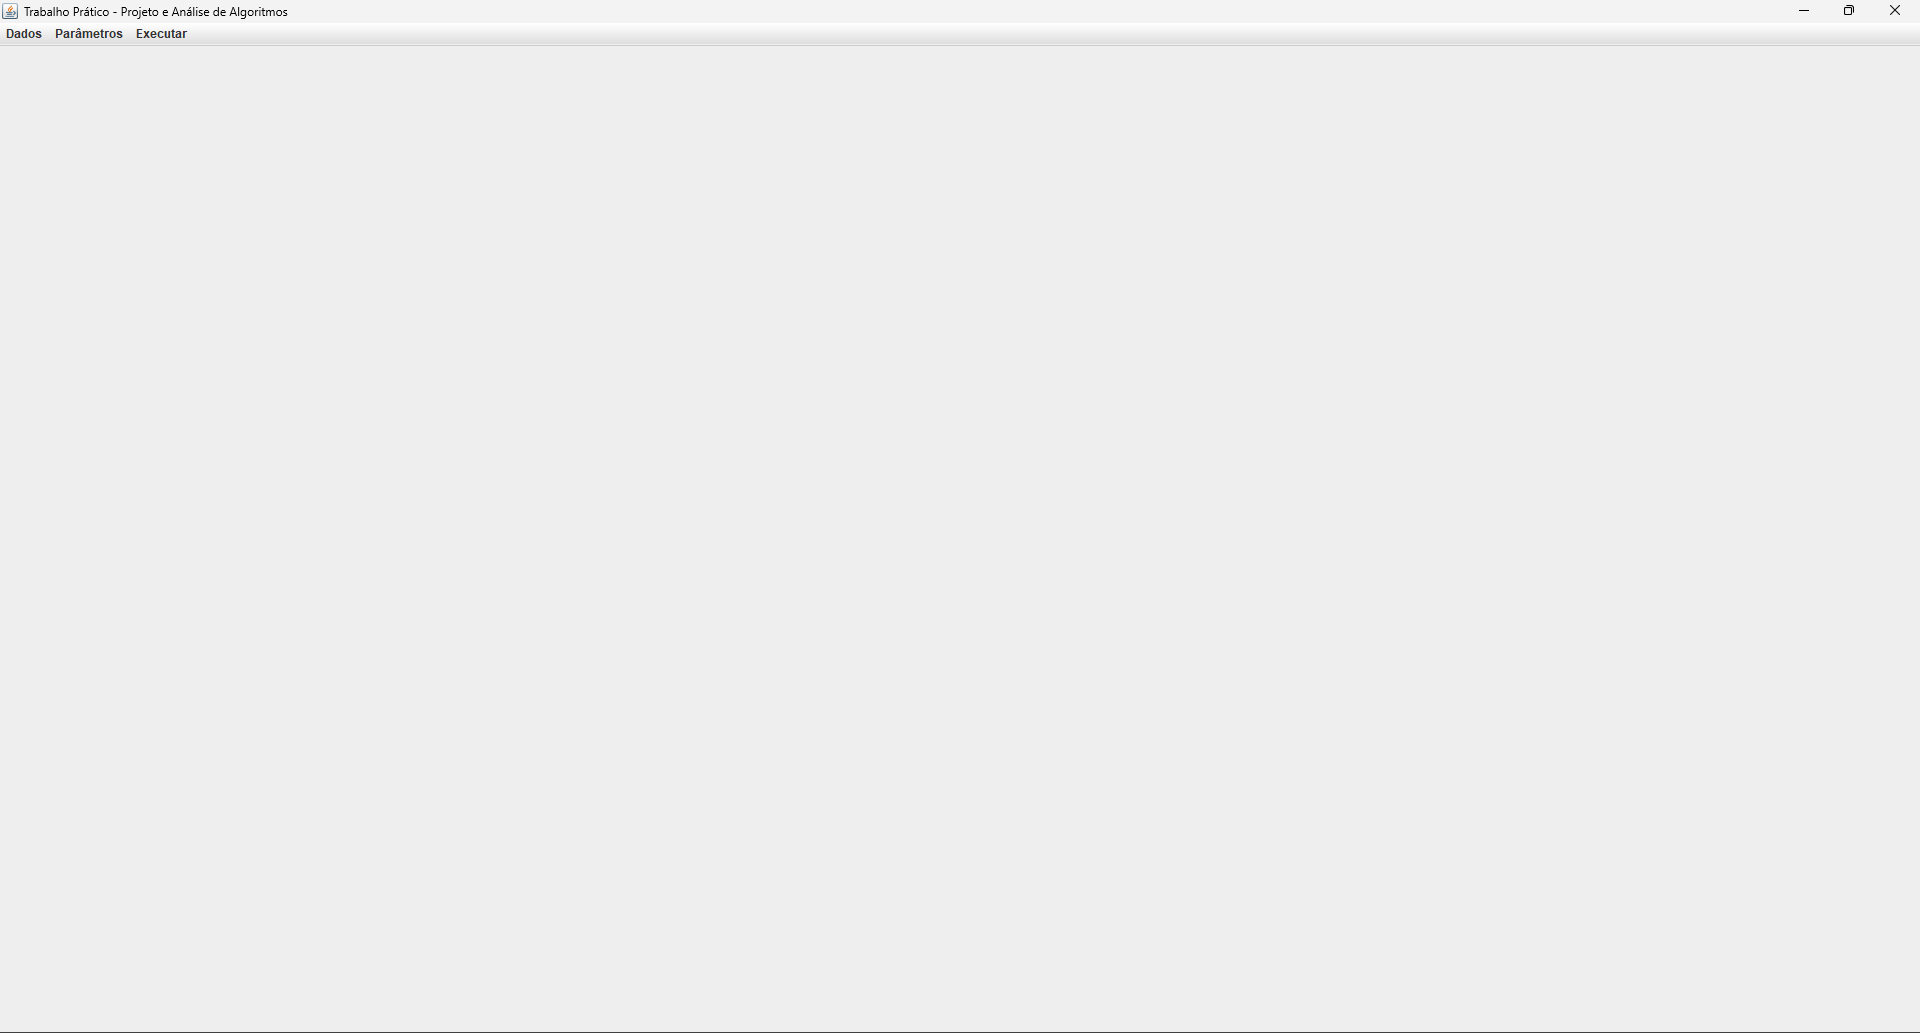
\includegraphics[width=\textwidth]{Captura de tela 2024-06-01 110824}
    \caption{Janela principal, quando o programa é iniciado}
    \label{fig:fig-1}
\end{figure}

\begin{figure}[H]
    \centering
    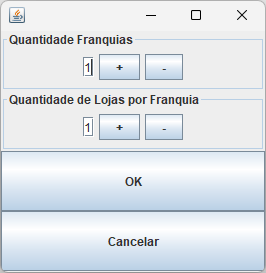
\includegraphics[width=\textwidth]{Captura de tela 2024-06-01 110836}
    \caption{Janela para a geração de dados aleatórios}
    \label{fig:fig-2}
\end{figure}

\begin{figure}[H]
    \centering
    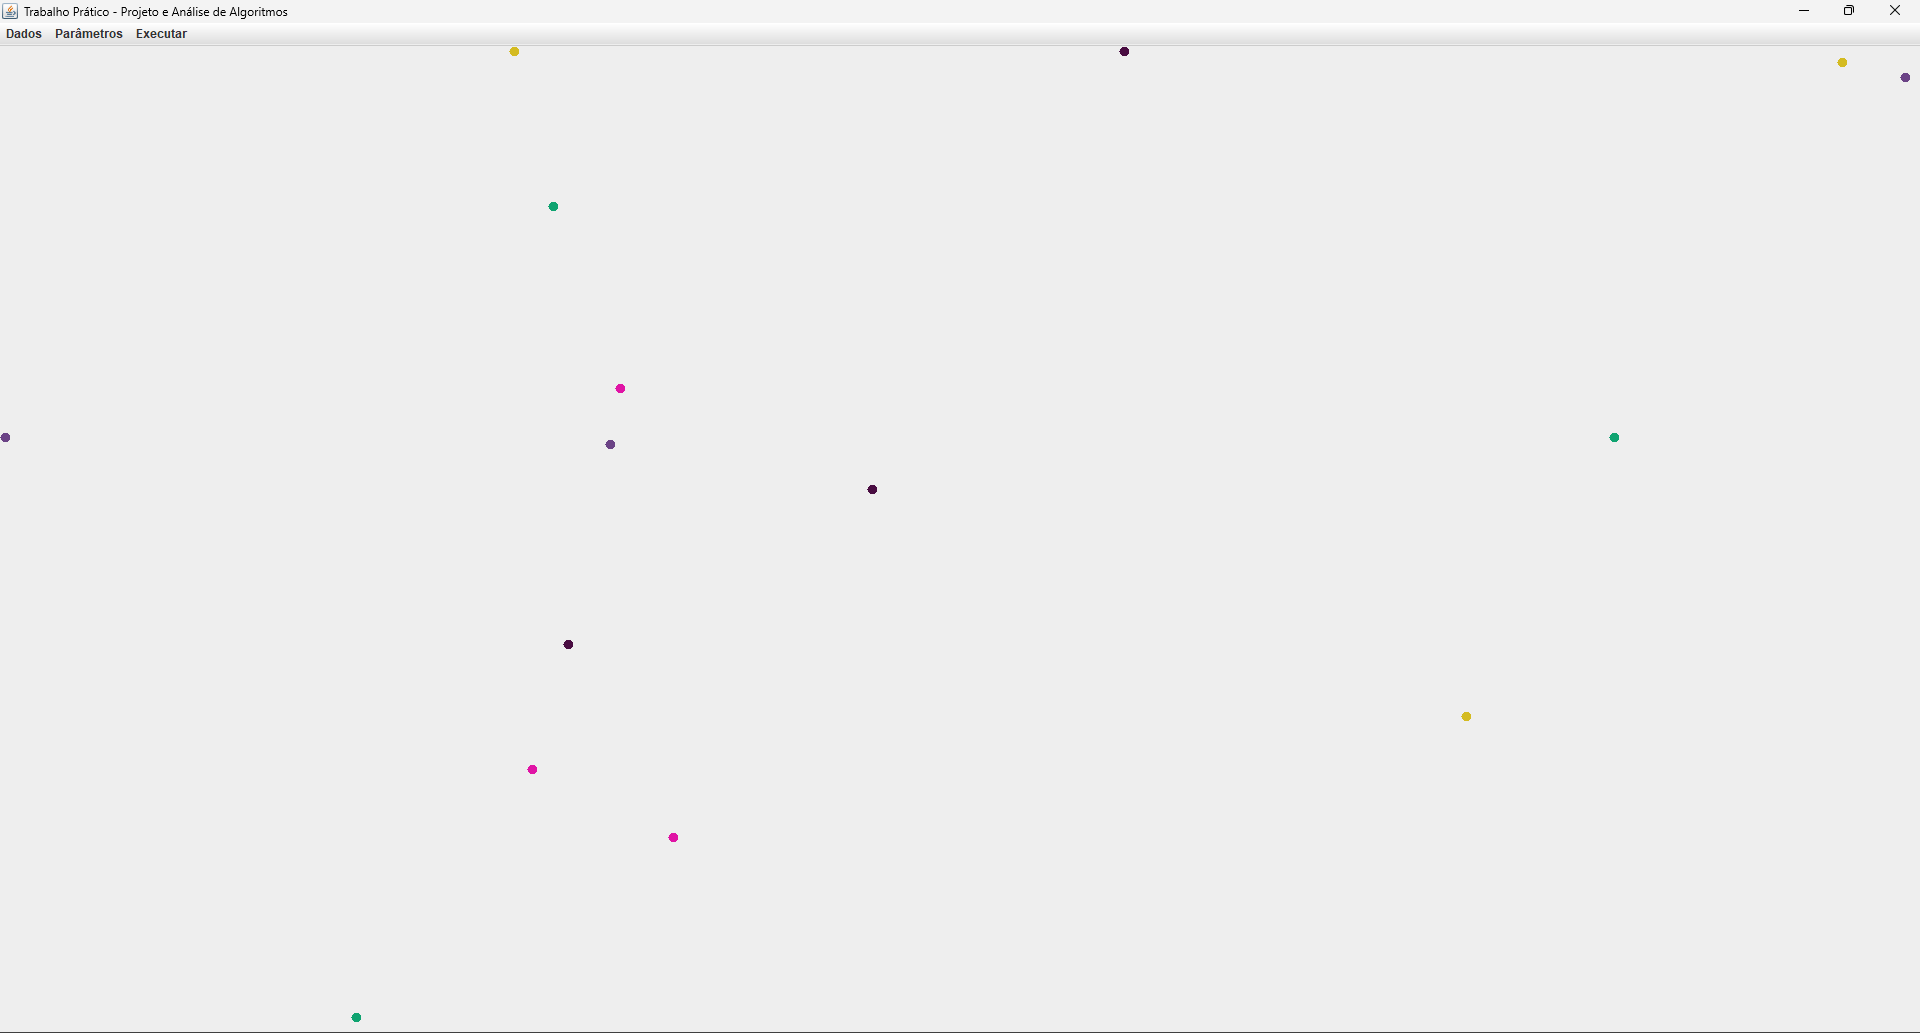
\includegraphics[width=\textwidth]{Captura de tela 2024-06-01 110914}
    \caption{Janela principal, mostrando o mapa de pontos escolhidos}
    \label{fig:fig-3}
\end{figure}

\begin{figure}[H]
    \centering
    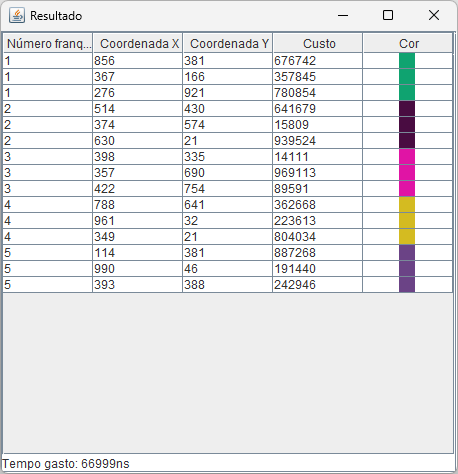
\includegraphics[width=\textwidth]{Captura de tela 2024-06-01 110920}
    \caption{Janela de resultados, mostrando a solução encontrada e o tempo gasto}
    \label{fig:fig-4}
\end{figure}

\begin{figure}[H]
    \centering
    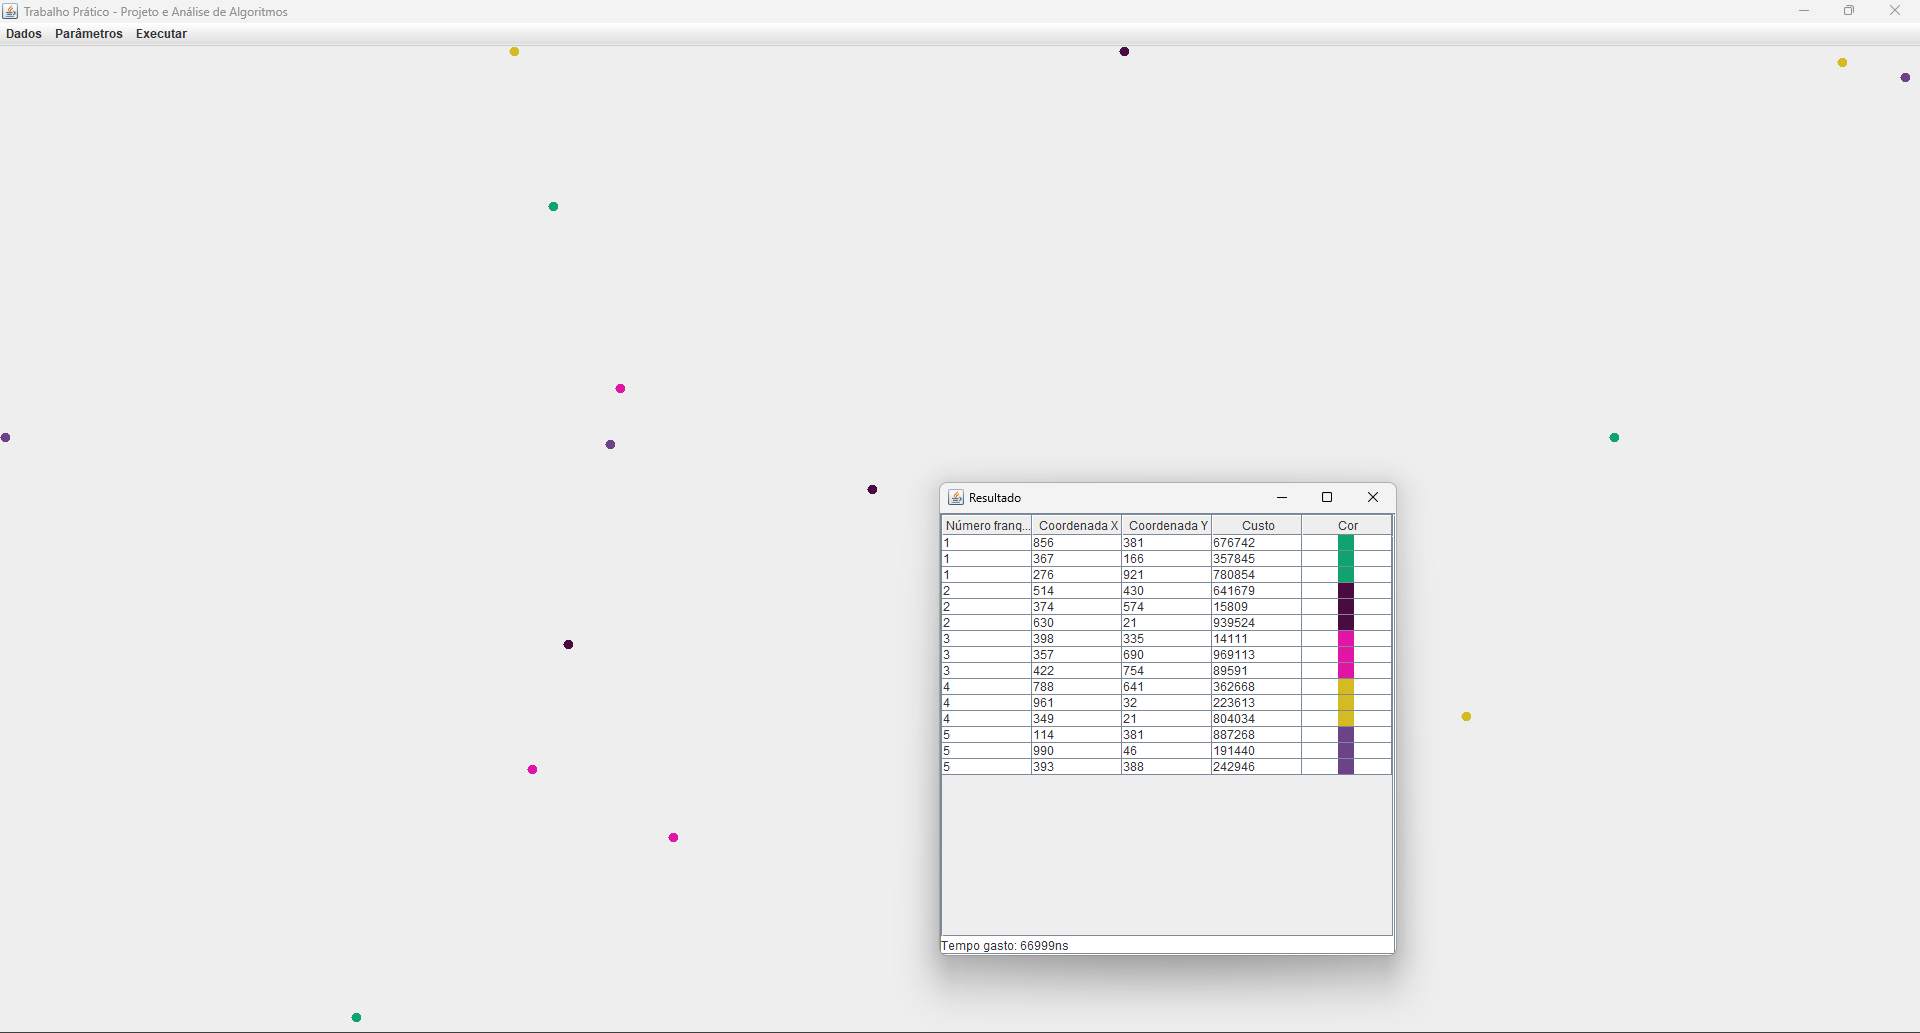
\includegraphics[width=\textwidth]{Captura de tela 2024-06-01 110931}
    \caption{Janela principal atrás da janela de resultados, mostrando o mapa, a solução encontrada e o tempo gasto}
    \label{fig:fig-5}
\end{figure}

\begin{figure}[H]
    \centering
    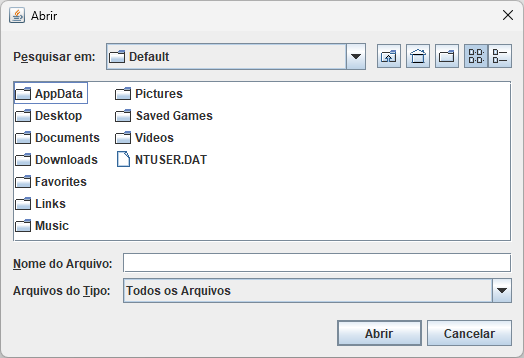
\includegraphics[width=\textwidth]{Captura de tela 2024-06-01 111051}
    \caption{Janela de abertura de arquivos}
    \label{fig:fig-6}
\end{figure}

\begin{figure}[H]
    \centering
    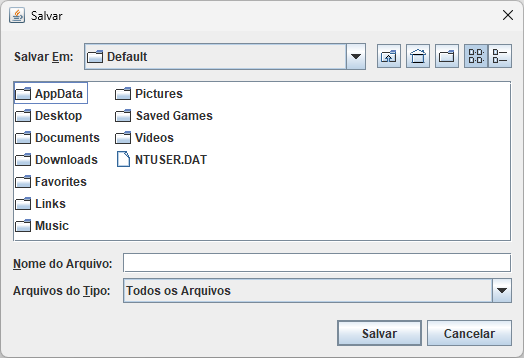
\includegraphics[width=\textwidth]{Captura de tela 2024-06-01 111107}
    \caption{Janela de salvamento de arquivos}
    \label{fig:fig-7}
\end{figure}

\begin{figure}[H]
    \centering
    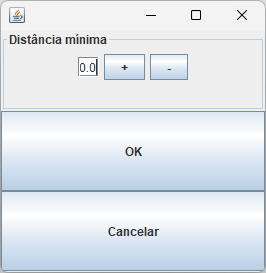
\includegraphics[width=\textwidth]{Captura de tela 2024-06-01 111132}
    \caption{Janela para a configuração da distância mínima permitida entre os pontos escolhidos}
    \label{fig:fig-8}
\end{figure}

\paragraph{}Além das janelas, também foi desenvolvida a opção de executar o programa por meio de argumentos de linha de comando, permitindo a realização de testes automatizados de desempenho e a coleta dessas métricas para a produção de gráficos. Para isso foi desenvolvido comandos e opções que devem ser passados por argumentos na execução do programa.

\paragraph{}Os comandos são: 

\begin{itemize}
    \item \textit{?}, \textit{-h}, ou \textit{\-\-help}, que exibe o menu de ajuda, permitindo o usuário entender o funcionamento o programa por linha de comando.
    \item \itemit{\-\-calcular-tempo}, que executa a função de cálculo de tempo de execução.
\end{itemize}

\paragraph{}As opções são:

\begin{itemize}
    \item \textit{\-\-arquivo-dados} <nome-arquivo-dados>, que especifica qual arquivo de dados deve ser aberto pelo programa.
    \item \textit{\-\-distancia-minima} <distancia-minima>, que especifica a distância mínima permitida entre os pontos escolhidos.
    \item \textit{\-\-algoritmo} <nome-algoritmo>, que define qual algoritmo de otimização deve ser utilizado: \textit{branch-and-bound} ou \textit{forca-bruta}.
\end{itemize}

\paragraph{}Para a validação do funcionamento dos algoritmos de otimização e os seus tempos de execução, foram desenvolvidos testes de unidades por meio do JUnit. Dentre os testes desenvolvidos estão:

\begin{itemize}
    \item \textit{testExemploProfessorRestricaoMaxima}, que executa o teste com os dados de exemplo do enunciado do trabalho, com a restrição (distância mínima permitida) máxima (300).
    \item \textit{testExemploProfessorMeiaRestricao}, que executa o teste com os dados de exemplo passados no enunciado do trabalho, com metade da restrição (150).
    \item \textit{testExemploProfessorNenhumaRestricao}, que executa o teste com dos dados de exemplo passados no enunciado, com nenhuma restrição (0).
    \item \textit{testAlgoritmosAleatoriamente}, que utiliza o \textit{Random} (com seed predefinida), para gerar os pontos candidatos.
    \item \textit{testAlgoritmosAleatoriamenteSeguro}, que utiliza o \textit{SecureRandom} (completamente aleatório), para gerar os dados dos pontos candidatos.
\end{itemize}

\section{Relatório de testes}

\paragraph{}Para a realização de testes de desempenho foi utilizado uma planilha no Jupyter, no qual era feita a execução do programa no modo linha de comando, passando o algoritmo de otimização, o arquivo de dados e a distância mínima permitida entre os pontos escolhidos, e era coletado à saída do programa com o tempo de execução gasto em nano-segundos pelo algoritmo. No final esses dados eram exportados em um arquivo Comma Separated Values (CSV). Em outra planilha, o arquivo CSV era importado, e seus dados eram processados para a geração de gráficos.

\paragraph{}Esse gráfico de barras comparanda a média dos tempos de execução dos algoritmos da Força Bruta e Branch and Bound. Nele é possível ver que o algoritmo Branch and Bound tem um desempenho médio um pouco melhor que o algoritmo da Força Bruta.

\begin{figure}
    \centering
    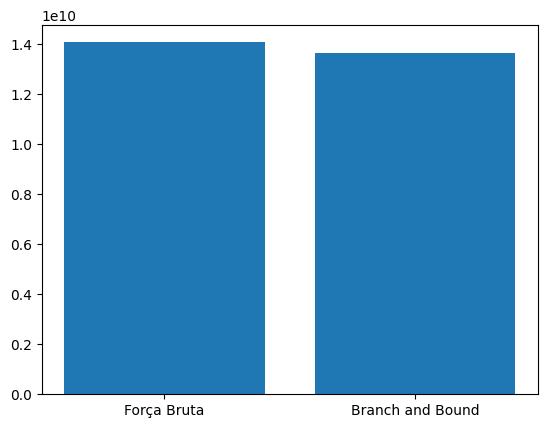
\includegraphics{comparacao.png}
    \caption{Gráfico de barras comparando a média do tempo de execução do algoritmo da Força Bruta e do Branch and Bound}
    \label{fig:fig-9}
\end{figure}


\paragraph{}O segundo gráfico gerado, foi o gráfico de barras comparando a média dos tempos de execução dos algoritmos da Força Bruta e Branch and Bound. Nele é possível ver que o algoritmo Branch and Bound tem um desempenho médio um pouco melhor que o algoritmo da Força Bruta.

\section{Conclusão}

Neste estudo foi colocado em prática o desenvolvimento e a análise de algoritmos de otimização em um problema da vida cotidiana, demonstrando a importância do estudo, pesquisa e desenvolvimento de algoritmos eficientes para a resolução de problemas do dia a dia.

\section{Referencias Bibliográficas}



%\bibliographystyle{sbc}
%\bibliography{sbc-template}

\end{document}
